\documentclass{article}
\usepackage[utf8]{inputenc}
\usepackage{graphicx}

\title{Report Machine Learning Third Assignment}
\author{Stefano Branchi [207523] \\ stefano.branchi@studenti.unitn.it \\\\ University of Trento}
\date{}

\begin{document}

\maketitle

\begin{abstract}
    The report for the third assignment of Machine Learning. The aim of this assignment is to create a basic Neural Network for the task of the OCR (Optical Character Recognition). For the implementation I used Python 3, numpy and tensorflow.
\end{abstract}

\section{Dataset}
The structure of the OCR dataset is the following one:
\begin{itemize}
  \item \textbf{train-data.csv}\\ Training data set is composed by 41721 records, each record is the list of 0/1 bits composing a 16x8 image
  \item \textbf{train-target.csv} \\ Training target set is a list of character that each training data line references
  \item \textbf{test-data.csv} \\ It's composed by 10431 records and it has the same structure of the train data set
  \item \textbf{test-target.csv} \\ It has the same structure of the train target set
\end{itemize}

\subsection{Pre-processing}
Numpy arrays are create for each dataset without any cleaning step, then targets are encoded in the one-hot format. In this way the algorithm can take numerical data instead of categorical one that, in this case is alphabetical.

\section{Neural Network Structure}
The architecture of the Neural Network is the same as the one used in the laboratory class, so it has the architecture of the ReLu network proposed by the MNIST. The architecture is shown in Figure \ref{fig:mnist_deep}

\begin{figure}[ht]
  \centering
  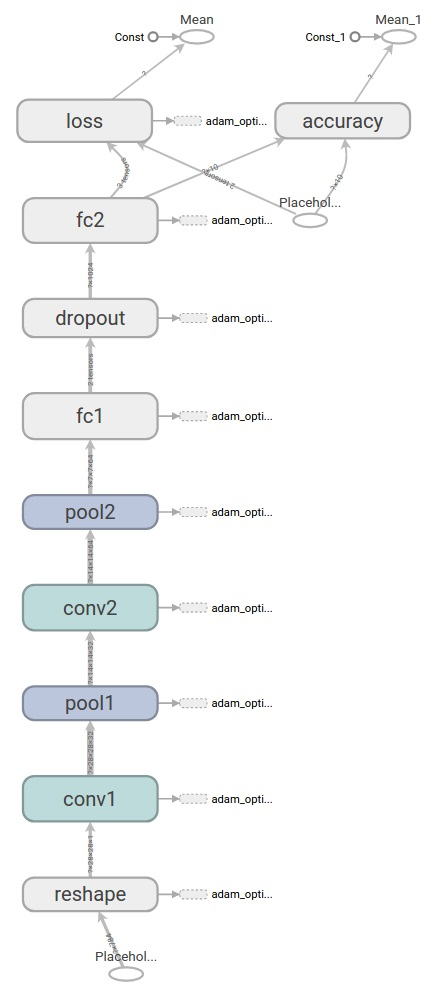
\includegraphics[scale=0.6]{images/mnist_deep.jpg}
  \caption{Architecture of the Neural Network}
  \label{fig:mnist_deep}
\end{figure}

\section{Final Results}
After the training and the validation of the Neural Network it achieves an accuracy of 75.40\% that is not a good result, but is above the baseline accuracy. To achieve better results it's possible to work on the architecture of the network to make possible a better feature extraction.
Training and testing results can be found in Figure \ref{fig:results}

\begin{figure}[ht]
  \centering
  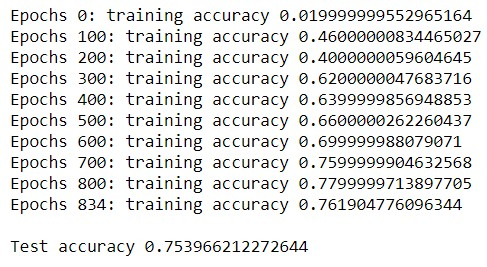
\includegraphics[scale=0.6]{images/results.jpg}
  \caption{Epochs and final result of the Network}
  \label{fig:results}
\end{figure}

\end{document}
